\documentclass{article}
\usepackage{graphicx}
\usepackage{amsmath,amsthm,amssymb}
\usepackage[font=small,labelfont=bf]{caption}
\usepackage{tikz}
\usetikzlibrary{calc, angles, quotes, shapes.geometric}
\usepackage{tkz-euclide}
\usepackage{float}
\usepackage[margin=1in]{geometry}
\usepackage{gensymb}
\usepackage{hyperref}
\hypersetup{
    colorlinks=true,
    linkcolor=blue,
    filecolor=magenta,      
    urlcolor=cyan,
    pdftitle={Overleaf Example},
    pdfpagemode=FullScreen,
    }
\usepackage{fancyhdr}
\pagestyle{fancy}
\fancyhead[R]{Enoch Yu}
\pagenumbering{gobble}
\usepackage{enumitem}
\newtheorem{theorem}{Theorem}[section]
\newtheorem{lemma}[theorem]{Lemma}
\newtheorem*{lemma*}{Lemma}
\newtheorem{sublemma}{Lemma}[section]
\newtheorem{proposition}{Proposition}
\newtheorem{corollary}{Corollary}[theorem]
\newenvironment{solution}{\begin{trivlist}\item[]{\bf Solution}}{\qed \end{trivlist}}
\newcommand{\verteq}{\rotatebox{90}{$\;\;=\;\;$}}
\newcommand*\circled[1]{\tikz[baseline=(char.base)]{
            \node[shape=circle,draw,inner sep=1pt] (char) {#1};}}
\newcommand{\triangled}[1]{\tikz[baseline=(char.base)]{
            \node[shape=regular polygon, regular polygon sides=3, draw, inner sep=0.2pt] (char) {#1};}}

\title{Problem Set 12}
\author{Enoch Yu}
\date{May 2025}

\begin{document}

\section*{Dependent Variable \& Independent Variable}
\textbf{Dependent Variable} \\
Variables \textbf{depends} on each other!! \\
For instance, if $x+y=10$, one variable depends on the value of another.
\\\\
\textbf{Independent Variable} \\
Variables \textbf{does not depend} on each other!! \\
For instance, if $1<x<7$ and $2<y<5$, the change in a variable does not affect the other.
\\\\
Dependent variables often form functions such as a linear function. However, independent variables form $x-axis$ and $y-axis$.

\section*{Problem}
You have a flight on Air China from Beijing to New York. The flight will depart any time between 1 p.m. and 6 p.m., uniformly at random. Your friend, Henry, is flying American Airlines, also from Beijing to New York. Henry's flight will depart any time between 3 p.m. and 5 p.m., uniformly at random. What is the probability that Henry's flight departs before your flight?
\begin{solution}
\\\\
\textbf{Key Word} Independent Variables
\\\\
First and foremost, Henry and I both depart uniformly at random. Meaning, the departure time of one does not affect the other, and independent variables could be assigned to each person.
\begin{center}
    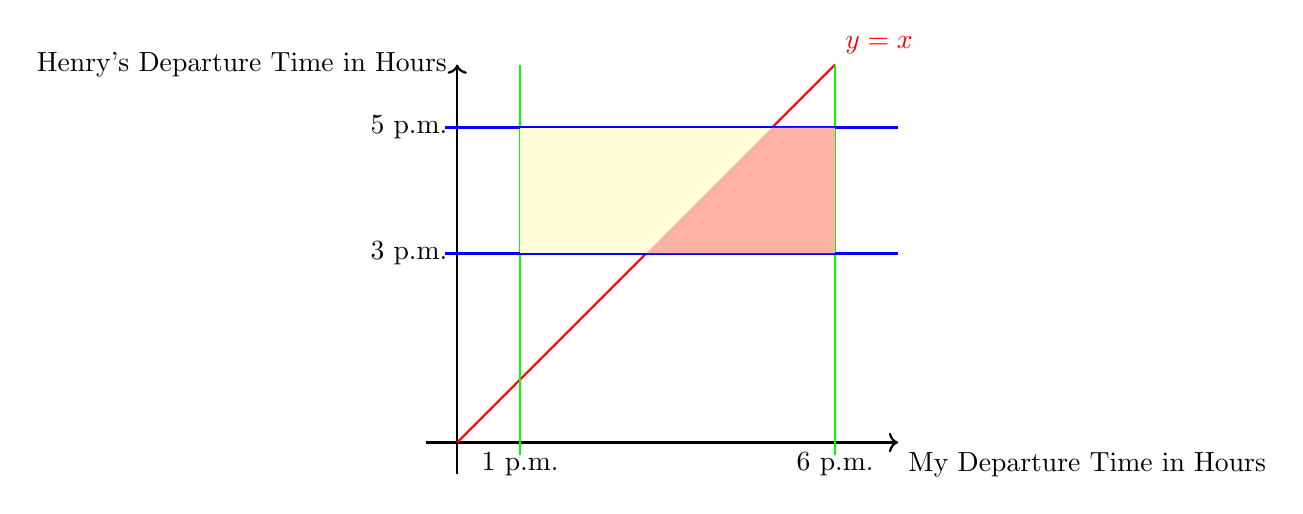
\begin{tikzpicture}[scale=0.8]
      \draw[->, thick] (-0.5,0) -- (7,0) node[below right] {My Departure Time in Hours};
      \draw[->, thick] (0,-0.5) -- (0,6) node[left] {Henry's Departure Time in Hours};
    
      \draw[red, thick] (0,0) -- (6,6) node[above right] {$y=x$};
    
      \draw[green, thick] (1,-0.2) -- (1,6);
      \draw[green, thick] (6,-0.2) -- (6,6);
    
      \draw[blue, thick] (-0.2,3) -- (7,3);
      \draw[blue, thick] (-0.2,5) -- (7,5);
    
      \fill[yellow!15] (1,3) rectangle (6,5);
    
      \begin{scope}
        \fill[red!50, opacity=0.6] (3,3) -- (5,5) -- (6,5) -- (6,3) -- cycle;
      \end{scope}

      \node[below] at (1,0) {1 p.m.};
      \node[below] at (6,0) {6 p.m.};
      \node[left] at (0,3) {3 p.m.};
      \node[left] at (0,5) {5 p.m.};
    \end{tikzpicture}
\end{center}
The enclosed rectangle colored in yellow provides every possible cases. Because the red linear line expresses times where Henry and I depart at the same time, the section colored in red provides time where Henry departs before my flight. Therefore, the probability may be found using the area of the colored sections.
\\\\
In the particular situation, groups of dots form a line and the lines form area since the end points are determined.
\\\\
\[
\frac{\text{Area of Section in Red}}{\text{Total Area}}=\frac{\frac{1}{2}\cdot2(1+3)}{2\cdot5}=\boxed{\frac{2}{5}}
\]
\end{solution}

\newpage
\section*{Problem}
Two mathematicians take a morning coffee break each day. They arrive at the cafeteria independently, at random times between 9 a.m. to 10 a.m., and stay for exactly $m$ minutes. The probability that either one arrives while the other is in the cafeteria is $40\%$, then find the value of $m$.
\begin{solution}
\\\\
\textbf{Key Word} Independent Variable
\\\\
Because both mathematicians arrive at the cafeteria independently, independent variables could be assigned for both mathematicians $A$ and $B$.
\begin{center}
    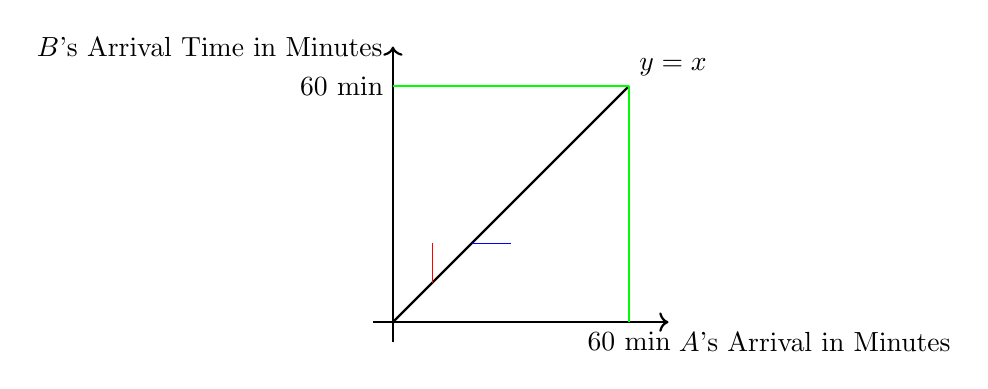
\begin{tikzpicture}[scale=0.5]
      \draw[->, thick] (-0.5,0) -- (7,0) node[below right] {$A$'s Arrival in Minutes};
      \draw[->, thick] (0,-0.5) -- (0,7) node[left] {$B$'s Arrival Time in Minutes};
    
      \draw[black, thick] (0,0) -- (6,6) node[above right] {$y=x$};
      \draw[green, thick] (6,0) -- (6,6);
      \draw[green, thick] (0,6) -- (6,6);

      \draw[red] (1,1) -- (1,2);
      \draw[blue] (2,2) -- (3,2);

      \node[below] at (6,0) {60 min};
      \node[left] at (0,6) {60 min};
    \end{tikzpicture}
\end{center}
The segment of $y=x$ manifests the time when both mathematicians arrive at the cafeteria at the same time. Moreover, WLOG, any points in the red and the blue segments with length of $m$ is valid because time flows equally for both mathematicians and the end points are the case when a mathematician meets the another while entering and leaving.
\begin{center}
    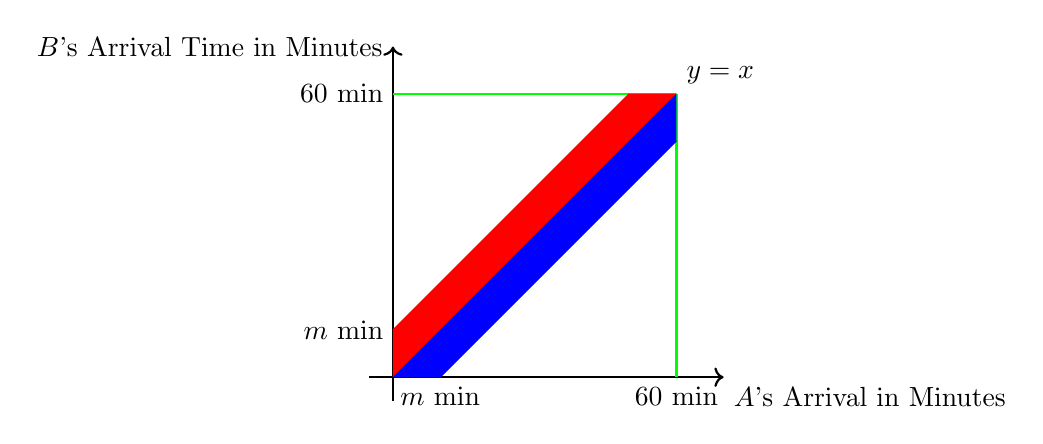
\begin{tikzpicture}[scale=0.6]
      \draw[->, thick] (-0.5,0) -- (7,0) node[below right] {$A$'s Arrival in Minutes};
      \draw[->, thick] (0,-0.5) -- (0,7) node[left] {$B$'s Arrival Time in Minutes};
    
      \draw[black, thick] (0,0) -- (6,6) node[above right] {$y=x$};
      \draw[green, thick] (6,0) -- (6,6);
      \draw[green, thick] (0,6) -- (6,6);

      \draw[red] (0,1) -- (5,6);
      \draw[blue] (1,0) -- (6,5);
    
      \begin{scope}
        \fill[red] (0,0) -- (0,1) -- (5,6) -- (6,6) -- cycle;
      \end{scope}
      \begin{scope}
        \fill[blue] (0,0) -- (1,0) -- (6,5) -- (6,6) -- cycle;
      \end{scope}

      \node[below] at (6,0) {60 min};
      \node[below] at (1,0) {$m$ min};
      \node[left] at (0,6) {60 min};
      \node[left] at (0,1) {$m$ min};
    \end{tikzpicture}
\end{center}
The colored area are the combination of all possible red and blue lines that were manifested without loss of generality. 
\begin{align*}
\frac{\text{Colored Area}}{\text{Total Area}}
=\frac{2\left[\frac{60\cdot60}{2}-\frac{(60-m)\cdot(60-m)}{2}\right]}{60\cdot60}&=\frac{40}{100} \\
\Rightarrow \frac{60\cdot60-(60-m)\cdot(60-m)}{60\cdot60}&=\frac{2}{5} \\
-5m^2+600m&=7200 \\
m^2-120m+1440&=0 \\
m&=60-\sqrt{2160} \ \text{ ($\because m<60$)} \\
&=\boxed{60-12\sqrt{15}}
\end{align*}
\end{solution}

\newpage
\section*{Problem}
In triangle $ABC$, $\angle{ABC}=120^{\circ}$. The internal bisector of $\angle{B}$ meets $AC$ at $D$. If $BD=1$, find the smallest possible value of $4BC+AB$.
\begin{solution}
\\\\
\textbf{Key Word} Triangle Area Formula, AM-GM Inequality
\\\\
First, graphing is required to understand the situation.
\begin{center}
    \begin{tikzpicture}[scale=0.6]
        \coordinate (A) at (-4,0);
        \coordinate (B) at (0,4);
        \coordinate (C) at (7,0);
        \coordinate (D) at (0.64,0);

        \draw (A) -- (B) -- (C) -- cycle;
        \draw (B) -- (D);

        \node[left] at (A) {$A$};
        \node[above] at (B) {$B$};
        \node[right] at (C) {$C$};
        \node[below] at (D) {$D$};
        \node[left] at ($(B)!0.5!(D)$) {$1$};

        \draw pic[draw=black, radius=0.2cm, "$120^{\circ}$", angle eccentricity=1.4] {angle=A--B--C};
    \end{tikzpicture}
\end{center}
Let $AB=a$ and $BC=b$. Angle and lengths are known. What can we do? We can use area!! Using the area formula of a triangle, the following equation is true.
\[
\frac{1}{2}\cdot\sin60^{\circ}\cdot{a}\cdot1+\frac{1}{2}\cdot\sin60^{\circ}\cdot{b}\cdot1=\frac{1}{2}\cdot\sin120^{\circ}\cdot{ab}
\]
In simpler terms, $a+b=ab$.
\\\\
Maximum value of $4a+b$ must be found using the fact that $a+b=ab$. First, $b=\frac{a}{a-1}$ is known. Therefore, the value could be substituted. Thus, the maximum value of $4a+\frac{a}{a-1}$ must be found.
\begin{align*}
4a+\frac{a}{a-1}
&=4a+1+\frac{1}{a-1} \\
&=4a-4+\frac{1}{a-1}+5 \\
&=4(a-1)+\frac{1}{a-1}+5 \\
\text{Using AM-GM Inequality, it is known that }& 4(a-1)+\frac{1}{a-1}\ge2\sqrt{4(a-1)\cdot\frac{1}{a-1}}=4. \\
\therefore\ &4+5=\boxed{9}
\end{align*}
\end{solution}

\end{document}
